\chapter{Approach and Results}\label{chap:chap4}


This chapter presents the main work which derived from the study performed in Chapter~\ref{chap:sota}. This includes the use cases that originated from having a web application that will be interacted with by the users. 

\section{Use Cases}\label{sec:use-cases}

As this project depicts the creation of a web application that users need to interact with, it is necessary to describe the possible scenarios that can arise, via use case diagrams.

\subsection{Search the existing VM images}\label{subsec:uc1}

\begin{figure}[h!]
  \begin{center}
    \leavevmode 
    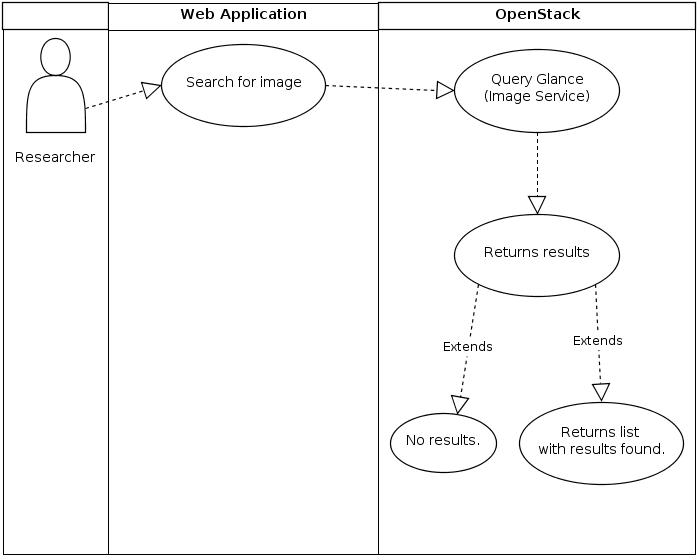
\includegraphics[scale=0.5]{uc1-search}
    \caption{Use Case 1: Search the existing VM images.}
    \label{fig:uc1-search}
  \end{center}
\end{figure}


\textbf{Actors}:

\begin{itemize}
\item Researcher.
\end{itemize}\ \\
\textbf{Use Case description:} After the web application is accessed, the researcher will need to choose the appropriate option displayed --- ``Search for an image.''. The researcher will then be shown a search form, where he/she will need to input the search terms deemed fit for the researcher's needs.

The web application will connect with \textit{OpenStack's} image service (\textit{Glance}), which will search for the terms inputted by the researcher.
If one or more VM images are found according to what was inputted, the search term and a list of VM images are presented. The items in the list are clickable, which mean they link to the details of the VM images displayed.
If no images are found, a specific text is displayed warning the researcher.

This use case is shown in Figure~\ref{fig:uc1-search}.


\subsection{View all the available VM images}\label{subsec:uc2}
\begin{figure}[h!]
  \begin{center}
    \leavevmode 
    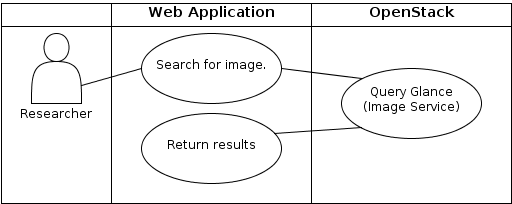
\includegraphics[scale=0.5]{uc2}
    \caption{Use Case 2: View all the available VM images.}
    \label{fig:uc2}
  \end{center}
\end{figure}
\textbf{Actors}:

\begin{itemize}
\item Researcher.
\end{itemize}\ \\
\textbf{Use Case description:} After the web application is accessed, the researcher will need to choose the appropriate option displayed --- ``View available images, details and statistics''. The researcher will then be shown a list of all the available images in the system.

This use case is shown in Figure~\ref{fig:uc2}.

\subsection{Create a VM image from scratch}\label{subsec:uc3}
\begin{figure}[h!]
  \begin{center}
    \leavevmode 
    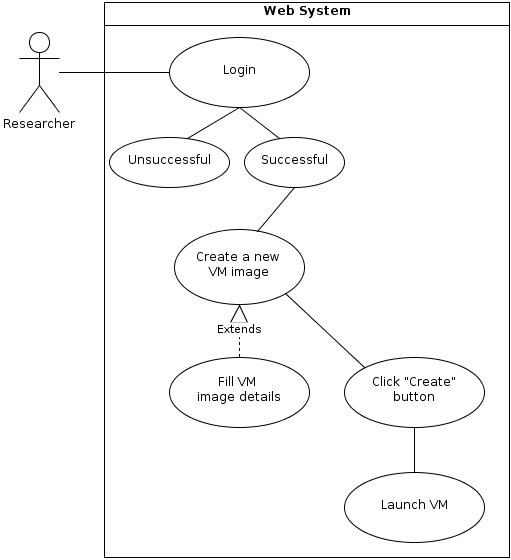
\includegraphics[scale=0.5]{uc3}
    \caption{Use Case 3: Create a VM from scratch.}
    \label{fig:uc3}
  \end{center}
\end{figure}
\textbf{Actors}:

\begin{itemize}
\item Researcher.
\end{itemize}\ \\
\textbf{Use Case description:} After the web application is accessed, the researcher will need to choose the appropriate option displayed --- ``Create an image suiting your needs (advanced)''. The researcher will then be shown a list of packages which will have a check box next to them. If the researcher wishes to include one package in the VM image to be created, he/she should click the check box next to the package name. 

This use case is shown in Figure~\ref{fig:uc3}.

A feature for including the packages outside the available list is discussed in Section~\ref{sec:future-work} - \nameref{sec:future-work}.


\subsection{Launching an already existing VM image}\label{subsec:uc4}
\begin{figure}[h!]
  \begin{center}
    \leavevmode 
    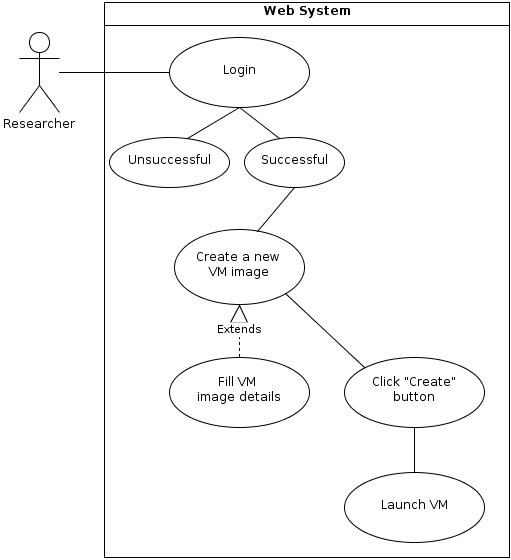
\includegraphics[scale=0.5]{uc3}
    \caption{Use Case 4: Launch an already existing VM image.}
    \label{fig:uc4}
  \end{center}
\end{figure}

\textbf{Actors}:

\begin{itemize}
\item Researcher.
\end{itemize}\ \\
\textbf{Use Case description:} After the web application is accessed, the researcher will need to choose the appropriate option displayed --- ``Use an already existing image.''. The researcher will then be shown a list of all the available VM images, from which he/she will be able to choose one for deployment. The web application will then connect with \textit{Glance}

This use case is shown in Figure~\ref{fig:uc4}.


\section{Implementation}\label{sec:implementation}


The application of the design and architecture described in Chapter~\ref{chap:chap3} is presented, being divided in three main areas:

\begin{itemize}
\item Cloud environment deployment (\textit{OpenStack});
\item Development of a web application;
\item Creation and management of VM images (communication between the two parts of the system mentioned in the previous bullet points).
\end{itemize}

\subsection{Cloud environment deployment}\label{subsec:cloud_env}

As mentioned in Chapter~\ref{chap:sota}, section~\ref{subsubsec:devstack}, \textit{DevStack} was used in order to simplify the cloud deployment.

Firstly, a clean installation of Ubuntu 12.04 LTS (as recommended by \textit{DevStack}' homepage) was created on Linux's \textit{Virtual Machine Manager} (\textit{libvirt}).

\textit{DevStack} deployment instructions were followed as they are in its webpage~\footnote{\url{http://devstack.org}} and after the script finished, the \textit{Horizon} Dashboard was accessible via a webpage, as it can be seen in Figure~\ref{fig:stack-dashboard}.

\begin{figure}[t]
  \begin{center}
    \leavevmode
    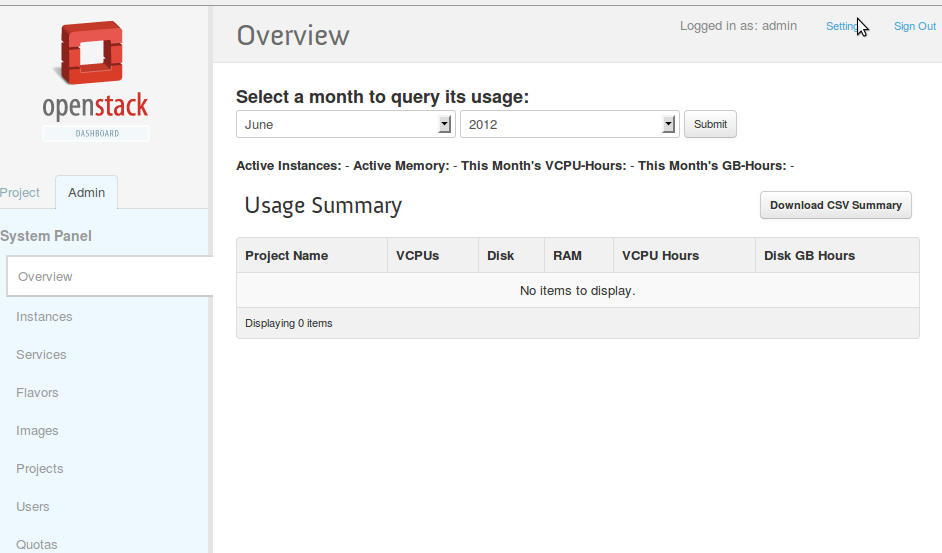
\includegraphics[width=\linewidth]{dashboard}
    \caption{\textit{OpenStack Horizon} Dashboard.}
    \label{fig:stack-dashboard}
  \end{center}
\end{figure}

All the desired services were up and running, as shown in Figure~\ref{fig:services}. Even though the image service (\textit{Glance}) was what was needed the most, it showed that the \textit{DevStack} deployment is a viable \textit{OpenStack} development tool.

\begin{figure}[h]
  \begin{center}
    \leavevmode
    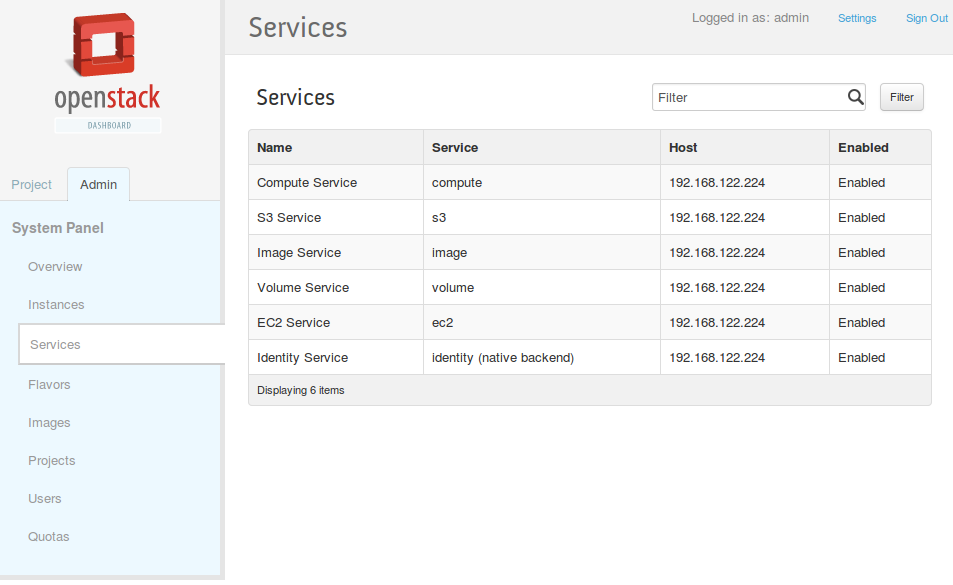
\includegraphics[width=\linewidth]{services}
    \caption{\textit{OpenStack} services.}
    \label{fig:services}
  \end{center}
\end{figure}

\subsection{Creation and management of VM images}\label{subsec:vm-create-manage}

As it was concluded in Chapter~\ref{chap:chap3} (~\nameref{chap:chap3}), the VM creation was implemented by using \textit{Ubuntu}'s \texttt{vmbuilder}. 

A \texttt{bash}~\footnote{Unix command shell.} script was created in order to automate the process. Since it is nothing more than a text file, it is easily modified by the \textit{Python} classes which are called by the web application. The user needs ``write'' permissions to run that file. An example of the script is attached in Appendix~\ref{chap:ap4} -~\nameref{chap:ap4}.

This script is run when the user finishes the VM image creating process in the web application.

\subsection{Web Applicationand VM image creation and contextualization}\label{subsec:webapp}

Since one of the goals of this project was to make submitting computing jobs an easier task, the web application was designed as simple as possible. The actions anyone is able to perform are limited to a bare minimum, while keeping the project's objectives in mind.

The user is only able to execute the following tasks:

\begin{itemize}
\item View all VM images available in the system;
\item Create a new VM image according to what the user needs --- limited to a set or pre-defined packages, due to the fact that packages can have long and sometimes not so obvious names;
\item Search for an existing VM in the system;
\item Use an already existing VM to be deployed.
\end{itemize}

This was explored in greater detail in the previous section, \nameref{sec:use-cases}.


The web application is fully developed in \textit{Python} and \textit{Django}. The searching of VM images is also built on \textit{Python} and one of its modules (\texttt{python-tagging}) is used. What the system currently does is assign a set of ``tags'' to the VM images. When the user uses the ``search'' function, the system is searching for these attacked tags. Should the user input match (partially or fully) any of the tags in the VMs, they will be returned in the final list.

The creation of VM images is made by using \texttt{vmbuilder}, which is called by using a \texttt{bash} script. This script is modified in real time by using the inputs from the user. The user chooses which packages to include in the VM image creation by selecting the appropriate boxes in the web application.

The script needs to be ran in \texttt{sudo} mode due to some restrictions enforced by the use of \texttt{vmbuilder}. In order to not compromise the server that runs the web application, the user will \textbf{only} be allowed to run this and only this script with \texttt{sudo} permitions.
To do this the \texttt{sudoers} file had to be altered in order to provide passwordless \texttt{sudo} access to the files in the scripts folder. 

One thing to have in mind is that the VM image creation process is very time consuming. Several tests were ran and the average time passed the twenty minute timeframe, on a small deployment (only \texttt{vim} and \texttt{openssh-server} were downloaded and installed). One of the script executions can be seen in Figure~\ref{fig:script-timer}.

\begin{figure}[h]
  \begin{center}
    \leavevmode
    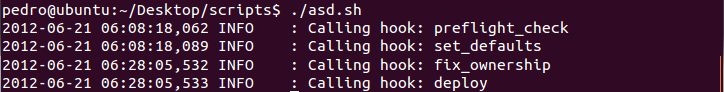
\includegraphics[width=\linewidth]{script-timer}
    \caption{One of the VM image creation test runs.}
    \label{fig:script-timer}
  \end{center}
\end{figure}

Connection with \textit{Glance} is made through a RESTful API. Communication with \textit{Glance} is established when the user wants to store a newly created VM image, wishes to use an already existing one and when the user wishes to view the images already stored in the server. This last case can be eliminated by storing the previous results on a text file, along with the timestamp of the last change made to that list (which should happen when a user creates and inserts a new VM image into the system).

Since the web application has \textit{Python} code on the background and \textit{OpenStack} is coded in the same programming language, this connection is seamless.

The modules \texttt{python-tagging} and \texttt{South} are needed for the web application to function properly. \texttt{python-tagging}, as it was mentioned earlier, is crucial for the search function, whereas \texttt{South} is used in database migrations.
\section{Conclusions}

This chapter presented how the architecture described in the previous chapter (\nameref{chap:chap3}) was implemented, as well as what were the use cases, the challenges encountered and if and how they were overcome. 
As for the goal completion, \textit{OpenStack} was fully deployed, as well as the web application. VM image creation was successful, as well as the contextualization process.
